%!TEX root = main.tex

\begin{frame}{Projector-based Analysis}{Tractability Index}
  % Is there a connection between the tractability index and the construction of projectors therein and the procedure using LU decompositions in Chapter 4?
  \begin{itemize}
    \item \textbf{Projector-based analysis} deals with properly stated leading term \acsp{DAE} of the form
    \begin{equation*}
      \m{F}(\m{d}(\mx, t)^\prime, \mx, t) = \m{0} % \m{A}(\mx, t)(\m{D}(t)\m{x})^\prime - \m{B}(\mx, t)
    \end{equation*}
    \item If we define the matrix sequence
    \begin{equation*}
      \begin{array}{l}
        \m{G}_0 = \m{A}\m{D} \quad \text{and} \quad \m{B}_0 = \m{B} \\
        \m{G}_{i+1} = \m{G}_i + \hlm{\m{B}_i \m{Q}_i} \\
        \m{B}_{i+1} = \left(\m{B}_i - \m{G}_{i+1}\m{D}^{-}\hlm{\frac{\text{d}}{\text{d}t}\left(\m{D}\m{P}_i\dots\m{P}_{i+1}\m{D}^{-}\right)}\m{D}\m{P}_i\dots\m{P}_{i-1}\right)\m{P}_i
      \end{array}
      \quad \text{with} \quad
      \begin{array}{l}
        \m{D} := \m{D}(\m{x}, t)        = \m{d}_{\m{x}}(\m{x}, t) \\
        \m{A} := \m{A}(\m{y}, \m{x}, t) = \m{F}_{\m{y}}(\m{y}, \m{x}, t) \\
        \m{B} := \m{B}(\m{y}, \m{x}, t) = \m{F}_{\m{x}}(\m{y}, \m{x}, t)
      \end{array}
    \end{equation*}
    and where $\m{P}_i = \m{I} - \m{Q}_i$, \quad $\m{Q}_i\m{Q}_j = \m{0}$, \quad $\m{D}^{-}\m{D} = \m{P}_0$
    \item The \textbf{tractability index} first integer $\mu$ where the matrix $\m{G}_\mu$ becomes non-singular
  \end{itemize}
  \hic{The difficult part is to compute the projectors $\m{Q}_i$}
\end{frame}

\begin{frame}{Projector-based Analysis}{Nnullspace Projectors}
  \begin{itemize}
    \item The \textbf{nullspace projector} $\m{Q}_i$ is found such that
    \begin{equation*}
      \hlm{\text{im}(\m{Q}_i) = \text{ker}(\m{G}_i)} \qquad
      (\m{G}_i\m{Q}_i = \m{0})
    \end{equation*}
    %\item The step $\m{G}_{i+1} = \m{G}_i + \m{B}_i \m{Q}_i$, is used to fill the matrix $\m{G}$ with the entries coming from the differentiated algebraic equations
    %\item The generalized inverse $\m{D}^-$ and the projector $\m{Q}_i$ are computed using matrix decomposition
    \item In \fullcite[ch.7, p.400]{lamour2013differential} is claimed that: \\[1.0em]
    \begin{quote}
      For problems of limited dimension a formula manipulation system like \Mathematica{} or \Maple{} can be used to compute a basis [of $\text{ker}(\m{Q})$]. The command in \Mathematica{} is \normalfont{\texttt{NullSpace[G]}} and in \Maple{} \normalfont{\texttt{nullspace(G)}}. \\
      However, to provide a basis of the nullspace of a given matrix one usually has to carry out a factorization, for instance a singular value decomposition (SVD).
    \end{quote}
  \end{itemize}
\end{frame}

%\begin{frame}{Q2 -- Gerdts}
%  How does the developed symbolic factorization method compare to GENDA by Mehrmann/Kunkel in view of CPU times?
%\end{frame}

%\begin{frame}{Q3 -- Gerdts}
%  The minimum degree pivoting strategy apparently worked for the examples in the thesis. In general, I assume, it cannot guarantee that all pivots are non-zero during evaluation. If a zero pivot is detected for a specific example, how would you proceed with the symbolic factorization?
%\end{frame}

%\begin{frame}{Q4 -- Gerdts}
%  Is it necessary to reduce to index-0 or would it be sufficient to reduce to index-1 and use a standard integrator like DASSL, RADAUIIA?
%\end{frame}

\begin{frame}{Projection and Consistent Initialization}{Projection Scheme}
  %Usually, there is no information related to all initial conditions, which must be calculated consistently. Do you think the index reduction strategy can be used to calculate consistent initial values?
  \begin{itemize}
    \item Same the \textbf{constrained minimization} problem
    \begin{equation*}
      \underset{\mx}{\text{minimize}} \quad \dfrac{1}{2}\left(\mx - \tilde{\mx}\right)^2 \quad \text{subject to} \quad \mhv = \m{0}
    \end{equation*}
    \item The \textbf{Lagrangian} of the minimization problem is
    \begin{equation*}
      \mathcal{L}(\mx, \boldsymbol{\lambda}) = \frac{1}{2}\left(\mx - \tilde{\mx}\right)^2 + \boldsymbol{\lambda} \cdot \mhv
      \quad \rightarrow \quad
      \begin{cases}
        \mx + \m{Jh}_\mx^\top \boldsymbol{\lambda} = \tilde{\mx} \\
        \mhv = \m{0}
      \end{cases}
    \end{equation*}
    \item The \textbf{iterative method} is \dots
    \begin{equation*}
      \begin{bmatrix}
        \m{I}        & \m{Jh}_\mx^\top \\
        \m{Jh}_{\mx} & \m{0}
      \end{bmatrix}
      \begin{bmatrix}
        \delta\mx \\
        \boldsymbol{\lambda}
      \end{bmatrix} = \begin{bmatrix}
        \tilde{\mx} - \mx \\
        -\mhv
      \end{bmatrix} \quad \text{where the step is} \quad \mx = \tilde{\mx} + \delta\mx
    \end{equation*}
    \item[] \dots derived from the Taylor expansion
    \begin{equation*}
      \begin{cases}
        \mx + \delta\mx + \m{Jh}_{\mx}^{\top}(\mx + \textcolor{mycolor2}{\delta \mx}, \m{v}, t) \boldsymbol{\lambda} = \tilde{\mx} \\
        \mhv + \m{Jh}_{\mx}(\mx, \m{v}, t) \delta\mx + \textcolor{mycolor2}{\mathcal{O}\left(\| \delta\mx \|^2\right)} = \m{0}
      \end{cases}
    \end{equation*}
  \end{itemize}
\end{frame}

\begin{frame}{Projection and Consistent Initialization}{Two Problems, One Solution}
  %Usually, there is no information related to all initial conditions, which must be calculated consistently. Do you think the index reduction strategy can be used to calculate consistent initial values?
  If part of ICs are not available:
  \begin{itemize}
    \item We can use the \textbf{projection scheme} to calculate consistent ICs
    \item The \textbf{iterative method} is reduced as selecting only the unknown ICs and the invariants we want to be maintained
  \end{itemize}
  \centering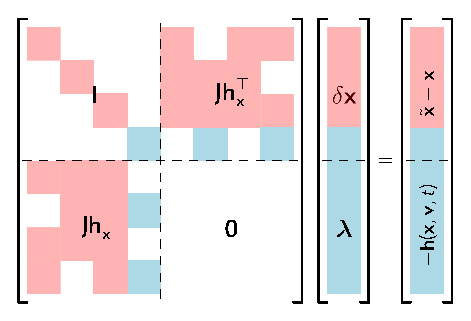
\includegraphics[width=0.5\textwidth]{initial_conditions.eps}
\end{frame}

%\begin{frame}{BVPs with DAEs}
%  %Do you think these techniques could be easily generalised to boundary value problems?
%  \begin{itemize}
%    \item \textbf{Single shooting} \\
%    \begin{small}
%      \qquad similar to the solution of IVPs\\
%      \qquad Jacobian matrix propagation might be influenced by the projection
%    \end{small}
%    \item \textbf{Multiple shooting} \\
%    \begin{small}
%      \qquad projection can be used at the junction points
%    \end{small}
%    \item \textbf{Collocation} \\
%    \begin{small}
%      \qquad remove some collocation point and add the projection to make the polynomial consistent with the invariants
%    \end{small}
%  \end{itemize}
%\end{frame}

% That's all Folks!